%Refraction
{
\psset{linestyle=none}
\textcolor{white}{\Large Refraction}

%Prism
\begin{itemize}
\item%
\begin{tabular}[t]{@{}l@{\hspace{0.1in}}l}%
	\begin{minipage}[t]{1.5in}\textcolor{white}{%
		Refraction, or bending of EMR, is dependent on wavelength. All wavelengths of EMR can be refracted by using the proper materials.
		White light can be spread by refraction into a spectrum of its composite colors with a glass prism.	
	% 	A right-angle prism will act as a mirror instead of a light refractor.  The critical angle of a true light-refracting prism is 42\degree.
		}%
	\end{minipage}&
	\raisebox{-0.8in}{\begin{minipage}[t]{1.42in}
		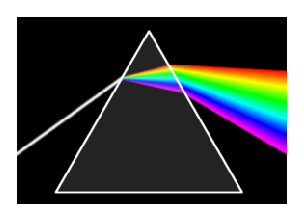
\includegraphics[scale=0.8]{pictures/prism.eps}
		\begin{center}Glass prism\end{center}
	\end{minipage}}
\end{tabular}

\item%
\begin{tabular}[t]{@{}l@{\hspace{0.1in}}l}%
	\begin{minipage}[t]{1.35in}{%
		Convex and concave lenses make objects appear closer and further and are used to correct far-sightedness and near-sightedness.
	}%
	\end{minipage}&
 	\raisebox{0.1in}
	{\begin{minipage}[t]{1.11in}%
		\rput(0.33,-.3){
			%Convex
			\psframebox{
				\psscalebox{0.9}{
					\psset{linestyle=solid,fillstyle=solid,fillcolor=darkgray}
					\psarc{c-c}(+.693,0){.8}{150}{210}
					\psarc{c-c}(-.693,0){.8}{330}{30}
					\psset{linestyle=solid,fillstyle=none}
					\psline{}(-.4,+.207)(-0.08,+.207)(.086,+.180)(.4,-.1)
					\psline(-.4,-.207)(-0.08,-.207)(.086,-.180)(.4,+.1)
				}
				\rput(0,-.4){\white Convex}
% 				\rput(0,-.47){\white lens}
			}
			%Concave
			\rput(0.68,0){
				\psframebox{
					\psscalebox{0.9}{
						\psclip{\psframe[fillstyle=none,linestyle=none,linearc=0,framearc=0](-.165,-.4)(.165,.4)}
						\psframe[fillstyle=solid,fillcolor=darkgray,linestyle=none,linearc=0,framearc=0](-.15,-.4)(.15,.4)
						\psset{linestyle=solid,fillstyle=solid,fillcolor=Black}
						\pscircle(+.85,0){.8}
						\pscircle(-.85,0){.8}
						\psline(-.157,-.389)(+.157,-.389)
						\psline(-.157,+.389)(+.157,+.389)
						\endpsclip
						\psset{linestyle=solid,fillstyle=none}
						\psline(-.4,+.180)(-0.086,+.180)(.08,+.207)(.4,+.4)
						\psline(-.4,-.180)(-0.086,-.180)(.08,-.207)(.4,-.4)
					}
					\rput(0,-.4){\white Concave}
% 					\rput(0,-.47){\white lens}
				}
			}
		}
	\end{minipage}}
	\end{tabular}

\item%
\begin{tabular}[t]{@{}l@{\hspace{0.14in}}l}%
	\begin{minipage}[t]{1.48in}\textcolor{white}{%
		Heavy objects like dense galaxies, stars, and large planets cause light to bend due to gravitational lensing as seen here in galaxy cluster Abell 2218:
		}%
	\end{minipage}&
	\raisebox{0.00in}{%
		\begin{minipage}[t]{1.16in}
			%http://imgsrc.hubblesite.org/hu/db/2004/08/images/a/formats/large_web.jpg
			\rput[tl]{90}(0,-.7){\textcolor{gray}{\footnotesize STScI}}
			\rput[tl]{0}(0.1,0.1){\includegraphics[width=1.18in]{pictures/gravlens.eps}}
		\end{minipage}
	}
\end{tabular}
	
\end{itemize}

}

%Gravity lens - manually drawn
%\psframebox{
%	\rput(-.75,0){
%		\PstStarFive[unit=.1,
%			fillstyle=solid,
%			fillcolor=white,
%			linestyle=solid,
%			linecolor=white,
%			PolyIntermediatePoint=0.3,
%			PolyRotation=45]
%	}
%	\pscircle[linestyle=solid,
%		linecolor=white,
%		fillstyle=solid,
%		fillcolor=Black](0,-.1){.2}
%	\pscurve[linestyle=solid,linecolor=white,fillstyle=none](-.6,.05)(0,+.15)(.6,.05)
%	\rput(.85,0){
%		\psclip{\psline[fillstyle=none,linestyle=solid,linecolor=white,linearc=0](.3;150)(0,0)(.3;210)}
%			\psclip{\pscircle[linestyle=solid,linecolor=white,fillstyle=solid,fillcolor=white]{.2}}% Eyeball
%			\rput(-.2,0){
%				\pscircle[fillstyle=solid,fillcolor=gray]{.10}% Iris
%				\pscircle[fillstyle=solid,fillcolor=Black]{.05}% Pupil
%			}
%			\endpsclip
%		\endpsclip
%	}
%}
